%!TEX root = ../main.tex
\section{Introduction}
This project is done in an effort to develop a double pendulum on a cart system for experimenting with control of unactuated systems.
In the first part of the report the inverted pendulum will be analysed in an effort to determine the requirements of a system capable of controlling such a pendulum system.
Electronics and mechanics will be developed to adhere to the found requirements and software will be written to serve as a base platform for the system.
Finally the report will be concluded with a verification and evaluation of every requirement of the designed system.

\subsection{System Overview} % (fold)
\label{sub:system_overview}
Since the reader is unlikely to have precognition of the report they are about to read, this section is written in an attempt to provide an overview of the terminology used going forward.
Figure \ref{fig:systemoverview} is a depiction of the finished design.
Every arrow points at a crucial part of the design which is referred to repeatedly throughout the report.
When the part is referred to it will be done by that name to limit any potential confusion.
\begin{figure}[h]
	\centering
	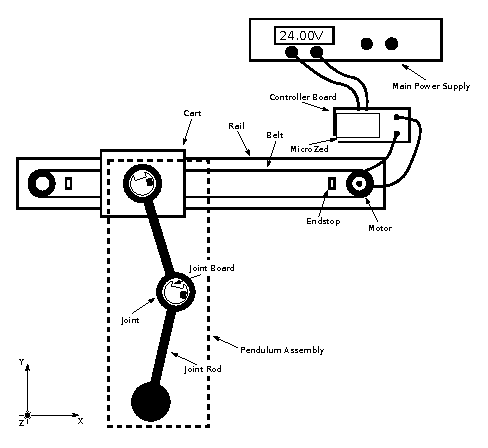
\includegraphics[width=\linewidth]{graphics/system_overview}
	\caption{Overview of the completed system.}
	\label{fig:systemoverview}
\end{figure}

Before you, the reader, fully embark on this journey, a few notes on the writing of this report. 
All component names, pin names, variables and states are written using the \texttt{teletype font}.
All components mentioned throughout the report will have the datasheet cited on the first mention of the component.
% subsection system_overview (end)

\subsection{System Users} % (fold)
\label{sub:system_users}
As will be elaborated on in future chapters, the system developed in this report is intended as an educational platform to be used in future projects.
It was proposed by the supervisor of the project, Leon Bonde Larsen who also set some of the requirements.
Throughout the report four types of actors are referred to:
\begin{itemize}
	\item \textbf{Project Owner:} The project owner, in this case also the supervisor, has proposed a system and also set certain requirements in the development of the system.
	In addition the project owner has been responsible for accepting any purchases made for the project. 
	\item \textbf{Authors:} Perhaps not surprisingly, this type refers to the authors of this report who, coincidentally, are also the original designers of the system.
	They are expected to have indepth knowledge of every aspect of the system.
	\item \textbf{Developers:} A developer is a person who does work to improve or otherwise alter the functionality of the system.
	They are expected to have knowledge of the interfaces that exist, both in hardware and software.
	Some developers may wish to further improve the electronics or joint design, however, for the purposes of this report, a developer is expected to use the hardware as-is.
	\item \textbf{User:} The user is a person who applies control algorithms to the system in an effort to balance the system.
	They are expected to have knowledge of the software interfaces related to motor control, system calibration and joint control.
\end{itemize}

% subsection system_users (end)